\documentclass[11pt,a4paper]{article}

% ---------------------------------------------------------------- packages
\usepackage[T1]{fontenc}
\usepackage[utf8]{inputenc}
\usepackage{charter}
\usepackage[a4paper,margin=1.15in]{geometry}
\usepackage{amsmath,amssymb}
\usepackage{graphicx}
\usepackage{booktabs}
\usepackage{tabularx}
\usepackage{enumitem}
\usepackage{xcolor}
\usepackage{fancyhdr}
\usepackage{titlesec}
\usepackage{caption}
\usepackage[hidelinks,backref=page]{hyperref}

\setlength{\parindent}{0pt}
\setlength{\parskip}{0.55em}
\setlist{itemsep=0.25em,topsep=0.3em}
\captionsetup{font=small,labelfont=bf}

\newcommand{\key}[1]{\textcolor{blue}{\textbf{#1}}}
\renewcommand*{\backref}[1]{}
\renewcommand*{\backrefalt}[4]{\ifcase #1 \or pages #2\else pages #2\fi}

% running header: current section on the right, like the review report
\pagestyle{fancy}
\fancyhf{}
\renewcommand{\headrulewidth}{0.4pt}
\renewcommand{\footrulewidth}{0.4pt}
\renewcommand{\sectionmark}[1]{\markright{\thesection\quad\MakeUppercase{#1}}}
\fancyhead[R]{\small\itshape\rightmark}
\fancyfoot[R]{\thepage}

\titleformat{\section}{\Large\bfseries}{\thesection}{1em}{}
\titleformat{\subsection}{\large\bfseries}{\thesubsection}{1em}{}

% ---------------------------------------------------------------- document
\begin{document}

\begin{titlepage}
\centering
\vspace*{2.2cm}
{\Large\textbf{ME303 - \textsc{Study Oriented Program}}\par}
\vspace{0.9cm}
{\Large BITS \textsc{Pilani}\par}
\vspace{0.3cm}
{\large \textsc{Department of CSIS}\par}
\vspace{1.4cm}
\rule{\linewidth}{0.8pt}\par\vspace{0.3cm}
{\huge\bfseries Value-Aware Adaptive Multi-Robot Exploration under Resource Constraints\par}
\vspace{0.3cm}
{\Large Semester Progress Report\par}
\vspace{0.2cm}
\rule{\linewidth}{0.8pt}\par
\vspace{1.8cm}
\begin{flushleft}
\textit{Author:}\\
Chaitanya Goyal (ID: 2024A7PS0557P)\\[0.8em]
\textit{Supervisor:}\\
Prof. Avinash Gautam\\
\vspace{3.2cm}
Date: November 2026
\end{flushleft}
\end{titlepage}

% ================================================================
\section{The Short Version}

This report is a check-in: what I have built so far, what I found, and where the project is going next.

In one paragraph: when a team of robots explores an unknown building, the first few minutes reveal a lot of new space, but the last few minutes are mostly long drives to find small leftover corners. Every minute still costs battery, messages between robots and planning time. So at some point, exploring more is not worth it. I built a small simulator to study this, taught a program to decide \emph{when} the team should stop, and tested whether that decision is actually worth learning. Following the review, the bigger goal is now to decide \emph{how much exploration effort} (how many robots, how much messaging) is still worth spending, with stopping being the case where zero robots keep working.

What I have so far:
\begin{itemize}
  \item \key{A working simulator} of robots exploring random buildings, with costs for driving, messages and planning.
  \item \key{A learned stop rule} that looks at the team's situation after every round and decides whether one more round is worth it.
  \item \key{Stage A done:} the problem is real. If robots explore until the map is complete, about a third of all their driving happens after the best moment to stop. But this is only true when driving and messaging are expensive.
  \item \key{Stage B done:} the reinforcement-learning way of training is clearly better than the obvious ``learn from the right answers'' way. A big model is not needed; even a simple one works.
  \item \key{A fair comparison} against five common stopping rules. In normal cases my rule ties the best one; in bad cases it loses far less.
  \item \key{All code and results} on GitHub, so everything can be re-run.
\end{itemize}

% ================================================================
\section{The Problem, in Plain Words}

\subsection{How robots explore a building}

Imagine the building as a big sheet of graph paper. Each square is either free space, a wall, or unknown. At the start, every square is unknown. Each robot can only see the squares near it (in my simulator, within 4 squares, and walls block the view).

A \key{frontier} is the edge between what we know and what we don't: a known free square right next to an unknown one \cite{yamauchi1997}. If a robot drives to a frontier, it gets to see new space. So exploration is basically: find frontiers, send robots to them, repeat. When there are several robots, each one should go to a different frontier so they don't waste effort on the same area \cite{burgard2005}.

I group the robots' work into \key{cycles}. One cycle is 6 robot steps: look around, share maps, pick frontiers, move. After every cycle, the team has a chance to decide: keep going, or stop?

\subsection{Why stopping is a real question}

The classic answer is ``stop when there are no frontiers left'', meaning the whole building is mapped. But look at what happens in practice (Figure~\ref{fig:tradeoff}). Early cycles reveal whole rooms. Later cycles reveal tiny pockets that need long drives. The cost keeps going up at roughly the same speed the whole time, but the new information slows down a lot.

\begin{figure}[h]
\centering
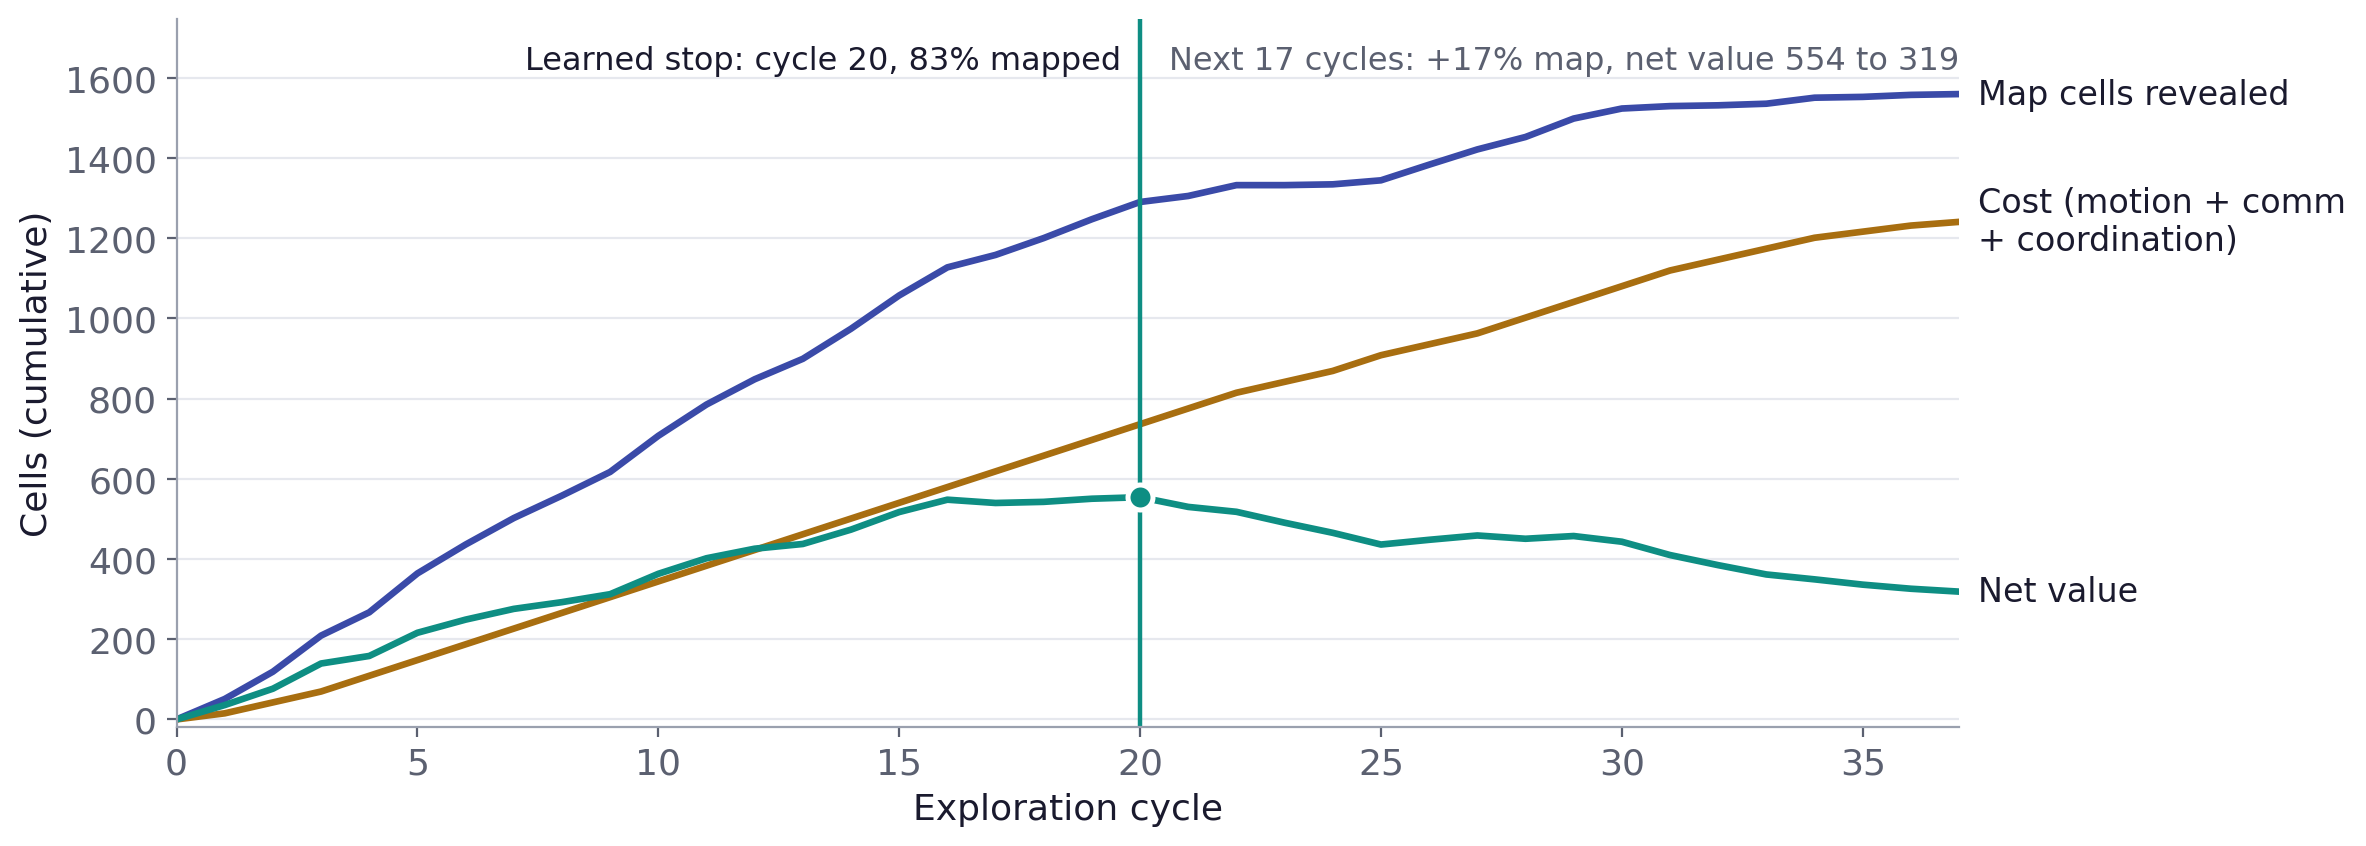
\includegraphics[width=\linewidth]{figures/fig_tradeoff.png}
\caption{One test run with 3 robots on a $40\times40$ map. Blue: total map found. Orange: total cost. Green: net value (map found minus cost). Net value peaks around cycle 20, when 83\% of the free space is mapped. The last 17 cycles add 17\% more map but drop the net value from 554 to 319.}
\label{fig:tradeoff}
\end{figure}

\begin{figure}[h]
\centering
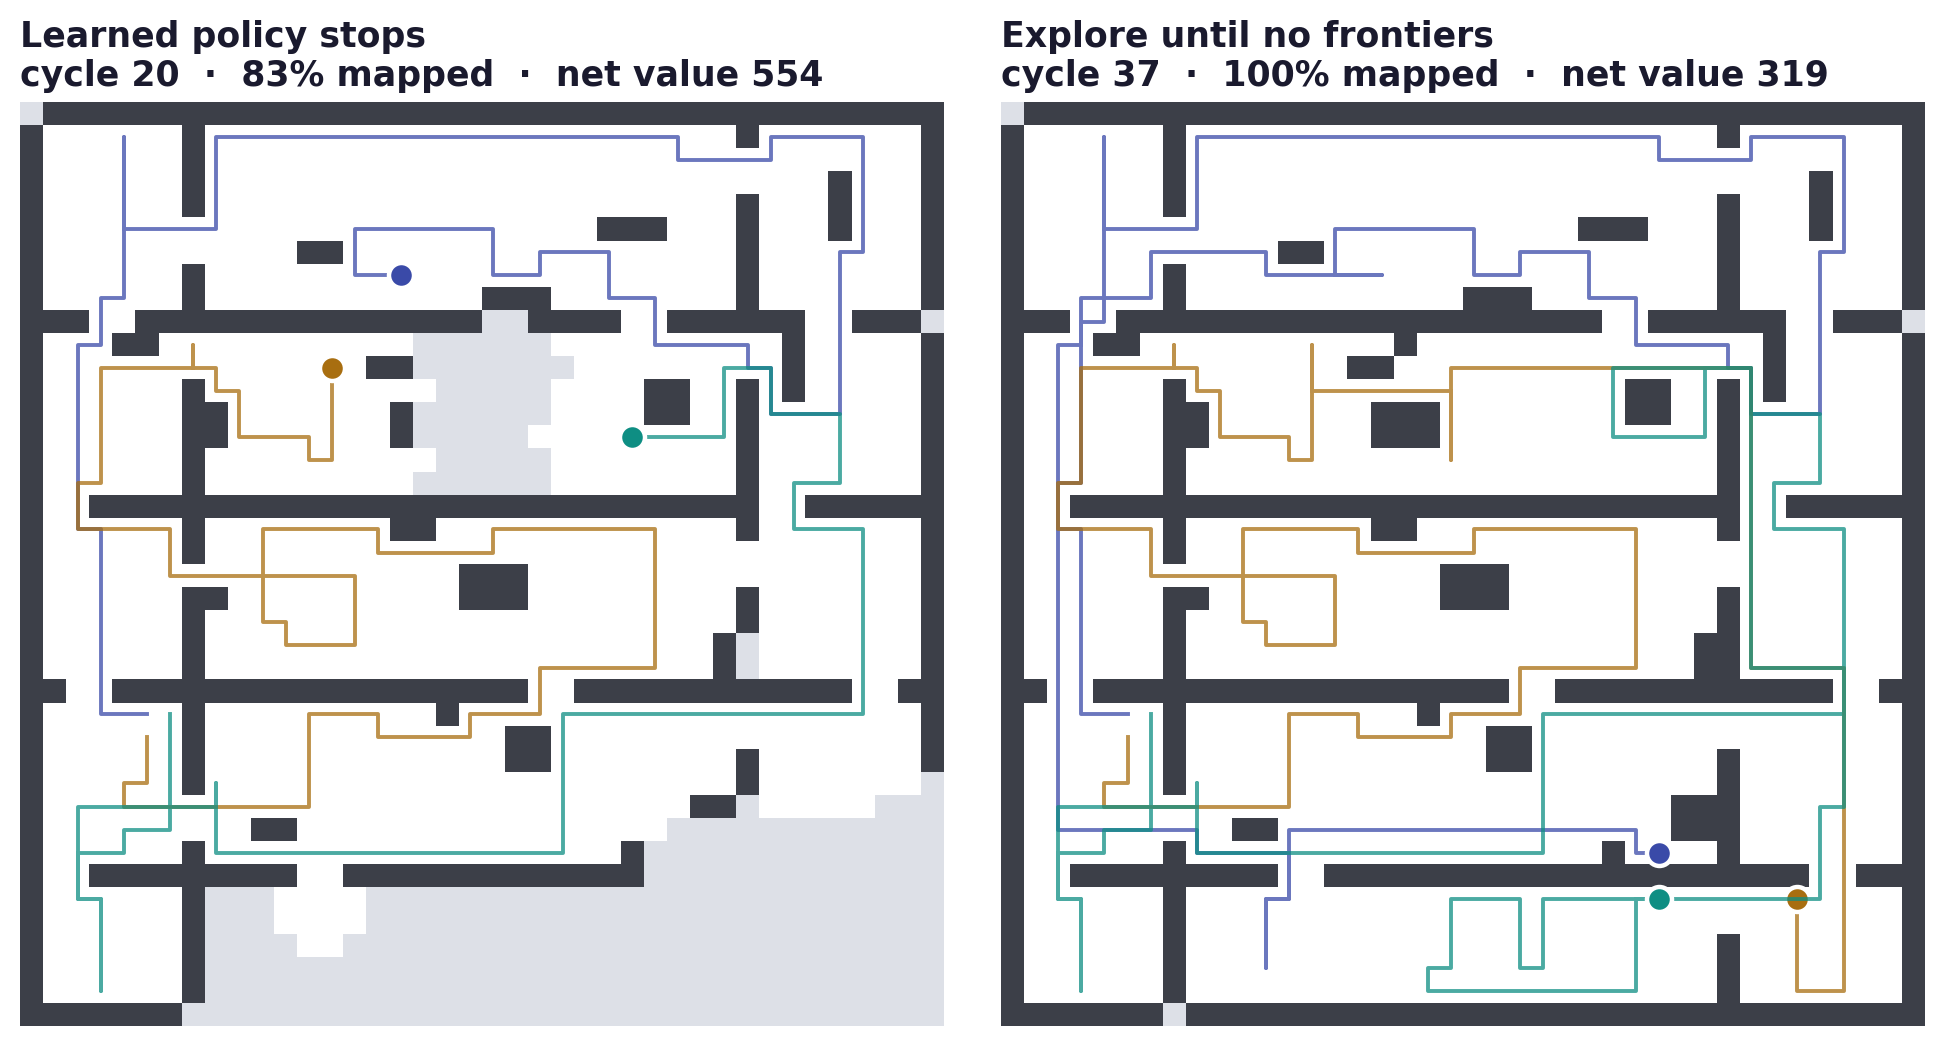
\includegraphics[width=0.92\linewidth]{figures/fig_maps.png}
\caption{The same map. Left: where the learned rule stopped (grey areas are still unknown). Right: exploring until nothing is left. The extra map on the right was expensive to get.}
\label{fig:maps}
\end{figure}

So the real question is not ``\emph{can} the team explore more?'' but ``\emph{is} one more cycle worth what it costs?''

\subsection{How I put a number on it}

To compare ``map found'' and ``cost'' I need them in the same units. I measure everything in map squares. The score of one cycle is:
\[
\text{score of a cycle} \;=\; \text{new squares seen} \;-\; c_{\text{move}}\cdot(\text{robot steps}) \;-\; c_{\text{comm}}\cdot N(N-1) \;-\; c_{\text{coord}}
\]
In words: what you found, minus what driving cost, minus what the messages cost (every one of the $N$ robots sends its map to every other robot, which is $N(N-1)$ messages), minus a fixed planning cost. By default I use $c_{\text{move}}=2$, $c_{\text{coord}}=2$, and a message cost of 0.05, 0.2 or 0.6 for cheap, medium and expensive messaging.

If you stop after $T$ cycles, your total is just the scores of those $T$ cycles added up. After a run is over, I can look back and find the cycle where this total was highest. I call that the \key{best stop in hindsight}. It needs knowledge of the future, so no robot could actually use it; it is only the 100\% mark I grade everything against.

% ================================================================
\section{What Changed After the Review}

The review raised two big points, and both changed the project.

\textbf{1. The original claim was too strong.} The first proposal said, roughly, that nobody had learned when a team of robots should stop exploring. The review pointed out papers that already deal with stopping exploration: Amorín et al.\ \cite{amorin2019} stop a whole robot team based on how much new information it is still expected to gain; Placed and Castellanos \cite{placed2022} stop a single robot when its uncertainty stops improving; Luperto et al.\ \cite{luperto2026} train a neural network to judge whether a map looks complete; PRoID \cite{kim2026proid} lets each robot decide when to go back and share its data; WiSER-X \cite{jadhav2026wiserx} lets each robot finish on its own schedule. None of them does exactly what I do, but together they mean ``stopping has not been studied'' is wrong.

So the claim is now narrower: \emph{to my knowledge, no earlier work \textbf{learns}, for the \textbf{whole team}, how much exploration effort is still worth spending, counting the costs of driving, messaging and coordination.}

\textbf{2. A yes/no stop does not justify a fancy two-level learning system.} If the only decision is ``continue or stop'', a professor could fairly ask: why not just use a simple threshold or a regression model? The review's answer is to make the top-level decision richer: instead of yes/no, decide \key{how many robots stay active}. For example, $8 \to 5 \to 2 \to 1 \to 0$. Stopping is then just the moment the number hits zero. This turns the project into a question about \emph{how much exploration effort is worth buying}, and it gives a real reason for two levels: the top level decides how much effort to spend, the bottom level decides how the remaining robots use it.

The review also asked for a step-by-step plan before any heavy machine learning (Stages A to E, Section~\ref{sec:plan}). I followed that order this semester.

% ================================================================
\section{What I Built}

Everything below is in the GitHub repository (\texttt{dev-goyal-chaitanya/marl-simulations}) and runs on a normal laptop.

\subsection{The simulator}
\begin{itemize}
  \item \textbf{Maps:} random indoor buildings on a grid: rooms, doors, and furniture blocks. Sizes $32\times32$, $48\times48$ and $64\times64$.
  \item \textbf{Robots:} 2 to 8 robots, all starting together. Each sees squares within 4 cells in line of sight.
  \item \textbf{Movement:} each robot drives to the nearest frontier, and robots are spread out so they don't chase the same one. This is a simple fixed rule. It is not what I am trying to improve; it is just the ``engine'' the robots run on.
\end{itemize}

\subsection{The learned stop rule}

The idea is simple. After each cycle, the team asks: \emph{if we keep going, how much net value do we expect to gain from here on?} Call that number $Q$. If $Q$ is zero or negative, stop.

Of course the team can't know the future, so a program has to \emph{estimate} $Q$ from what the team can see right now. I describe the team's situation with 7 simple numbers:
\begin{enumerate}
  \item how much of the map is already known,
  \item unknown squares near the planned targets, divided by the cost of one cycle,
  \item how well the last cycle paid off (gain divided by cost),
  \item how well the cycle before that paid off,
  \item how far away the planned frontiers are,
  \item what share of the robots still have somewhere to go,
  \item how much frontier is left, relative to the map size.
\end{enumerate}
All of them are fractions or ratios, not raw counts. That is on purpose: a ratio like ``gain per unit cost'' means the same thing for a small map and a big map, for 2 robots and for 8, so one rule can be used everywhere without retraining.

\subsection{How the program learns}

This is where reinforcement learning (RL) comes in. Put simply, RL means learning what to do from scores rather than from an answer key.

I used a method called \key{fitted Q-iteration} \cite{ernst2005}. Here is the whole idea:
\begin{enumerate}
  \item Run 300 practice maps (2 robots, $32\times32$) all the way to the end, and record the team's 7 numbers and the score of every cycle.
  \item Score each recorded run under 4 random sets of prices for driving, messages and planning. That gives 1,200 runs from the same 300, and stops the program from memorising one price.
  \item Start with a rough guess of $Q$. For every recorded moment, build a target: \emph{this cycle's score, plus the guessed value of the next moment (or 0 if it's better to stop there)}. Fit a model to those targets. That model is the new guess.
  \item Repeat step 3 twenty-five times. Each round, the guesses get better.
\end{enumerate}
The model in step 3 is an ``extra-trees regressor'': a group of 80 decision trees whose answers are averaged. It's fast and works well with small data.

The ``stop when the value of continuing is zero or less'' idea is old: it comes from finance, where people use it to decide when to cash in an option \cite{longstaff2001,tsitsiklis1999}. I am applying it to robot exploration.

\subsection{What I compare against}

A result means nothing without something to compare to. These are the rules I compare with:
\begin{itemize}
  \item \textbf{Explore until done:} stop only when no frontiers are left \cite{yamauchi1997,burgard2005}.
  \item \textbf{Fixed budget:} always stop after a set number of cycles (tuned to 19).
  \item \textbf{Coverage threshold:} stop once a set fraction of the grid is known (tuned to 84\%).
  \item \textbf{Myopic rule:} stop right after the first cycle that lost value.
  \item \textbf{Gain-vs-cost rule:} a hand-made rule that stops when the expected gain falls below the cycle cost divided by 1.6.
  \item \textbf{Best stop in hindsight:} the 100\% mark, not a real rule.
\end{itemize}
``Tuned'' means I picked the number that worked best on the training maps, which gives these rules a fair chance.

\subsection{How I judge results}

\begin{itemize}
  \item \textbf{\% of best:} total value a rule got, divided by the total value of the best stop in hindsight.
  \item \textbf{Value lost:} how much value a rule missed compared with the best stop, as a percentage of the map. This is more stable than ``\% of best'' when the best value is small.
  \item \textbf{Worst case:} the setting where a rule did worst. A rule that is fine on average but terrible somewhere is risky on a real robot.
  \item \textbf{Generalisation:} train once on 2 robots and small maps, then test on 36 different settings (2, 4, 6 or 8 robots; three map sizes; cheap, medium or expensive messaging; 40 maps each) \emph{without retraining}.
\end{itemize}
The way I report averages, worst cases and confidence ranges follows the advice in Agarwal et al.\ \cite{agarwal2021}, which is about how to compare learning methods honestly.

% ================================================================
\section{Results So Far}

\subsection{Stage A: is the problem even real?}

Before building anything clever, the review asked a simple question: \emph{how much value do we actually lose by exploring until the map is done?} If the answer is ``almost nothing'', the whole project is pointless.

I took 1,440 finished runs (the 36 settings above, 40 maps each), found the best stop in hindsight for each, and measured what the extra exploration cost.

\begin{figure}[h]
\centering
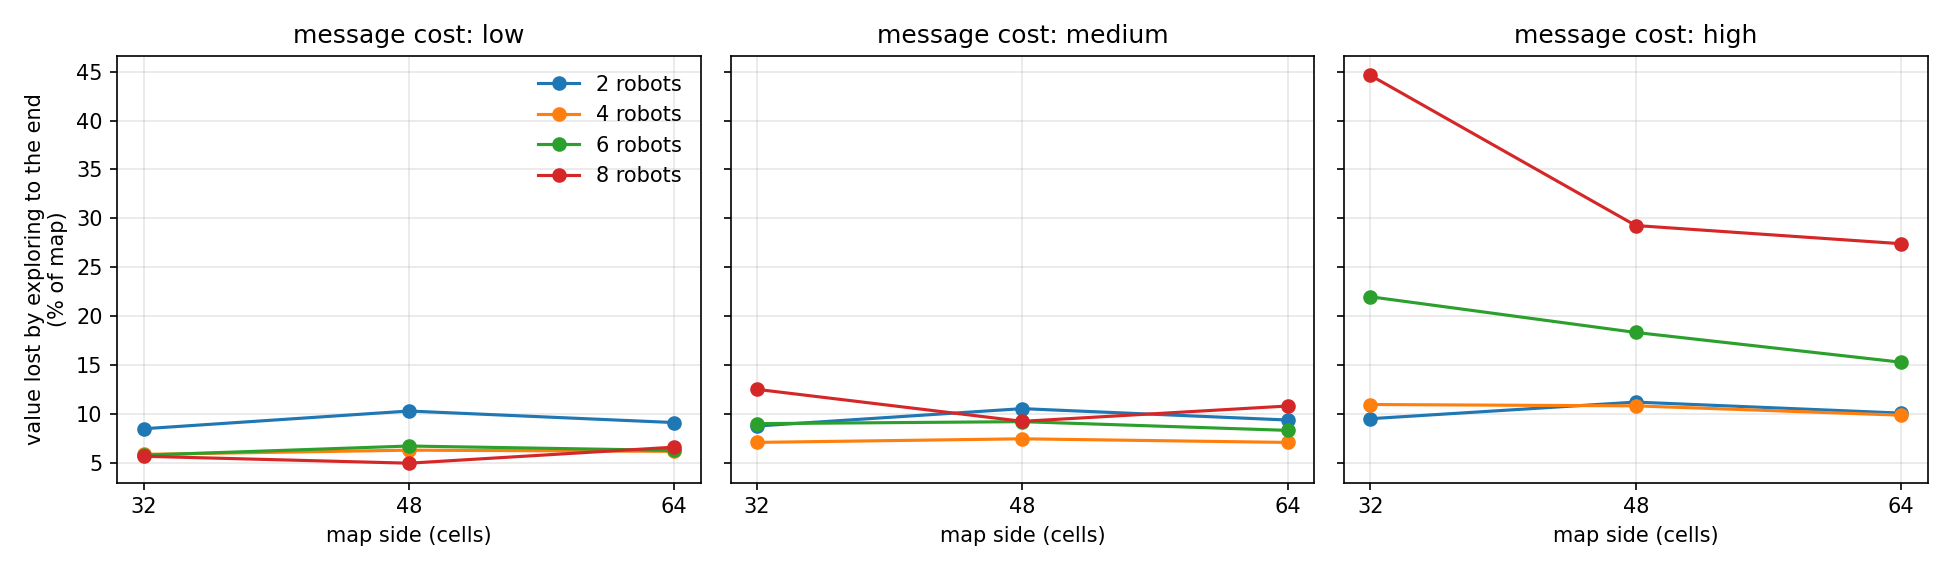
\includegraphics[width=\linewidth]{figures/week1_value_lost.png}
\caption{Value lost by exploring until done, as a percentage of the map. Each panel is one message cost; each line is a team size.}
\label{fig:stageA}
\end{figure}

\begin{table}[h]
\centering
\small
\begin{tabular}{lccc}
\toprule
Team size & Cheap messages & Medium & Expensive \\
\midrule
2 robots & 9.3 & 9.6 & 10.3 \\
4 robots & 6.1 & 7.2 & 10.6 \\
6 robots & 6.3 & 8.8 & 18.5 \\
8 robots & 5.8 & 10.8 & 33.8 \\
\bottomrule
\end{tabular}
\caption{Value lost by exploring until done (\% of map), averaged over the three map sizes.}
\label{tab:stageA}
\end{table}

What this shows:
\begin{itemize}
  \item On average, exploring until done throws away \key{11.4\% of the map's value}, and \key{36\% of all driving} happens after the best stopping point.
  \item It gets worse with \textbf{bigger teams} and \textbf{expensive messaging}. With 8 robots and expensive messages, a third of the value is lost.
\end{itemize}

\textbf{The honest catch.} All of this depends on how much I charge for driving. I re-scored the same runs with different driving prices (medium message cost):

\begin{table}[h]
\centering
\small
\begin{tabular}{ccc}
\toprule
Cost per robot step & Value lost (\% of map) & Driving after the best stop \\
\midrule
0.5 & 1.0 & 4.8\% \\
1 & 2.2 & 9.6\% \\
2 (default) & 9.1 & 33\% \\
3 & 27.3 & 68\% \\
\bottomrule
\end{tabular}
\caption{How the size of the problem depends on the price of driving.}
\label{tab:sens}
\end{table}

If driving is cheap, just explore everything; there is nothing to fix. The project matters when driving or messaging is expensive: big teams, small batteries, costly radio. So one of the next steps is to use realistic costs (from real robots), or to show results across the whole range.

\subsection{Stage B: do we actually need reinforcement learning?}

The review asked whether a simpler method would do. So I tried two ways of making the training targets, each with four kinds of model:
\begin{itemize}
  \item \textbf{RL-style (fitted Q-iteration):} the target uses the program's own estimate of what happens next, as described in Section~4.3.
  \item \textbf{Hindsight answers:} plain supervised learning. After each run, label every moment with the best value that was still possible from there, and train the model to predict that label. This looks like the obvious approach.
\end{itemize}

\begin{table}[h]
\centering
\small
\begin{tabular}{llccc}
\toprule
Training target & Model & Avg value lost & Worst setting & Settings $<$50\% \\
\midrule
\textbf{RL-style} & \textbf{extra trees} & \textbf{3.6} & \textbf{9.9} & \textbf{1} \\
RL-style & random forest & 3.7 & 10.3 & 1 \\
RL-style & linear & 3.5 & 13.0 & 4 \\
RL-style & neural net & 4.8 & 12.1 & 1 \\
Hindsight & linear & 6.7 & 30.4 & 6 \\
Hindsight & neural net & 5.4 & 37.4 & 5 \\
Hindsight & random forest & 9.0 & 35.7 & 8 \\
Hindsight & extra trees & 9.6 & 39.0 & 8 \\
\midrule
\multicolumn{2}{l}{Coverage threshold (tuned), for reference} & 4.7 & 25.3 & 5 \\
\bottomrule
\end{tabular}
\caption{Value lost (\% of map) over the 36 test settings, no retraining. Lower is better.}
\label{tab:stageB}
\end{table}

\begin{figure}[h]
\centering
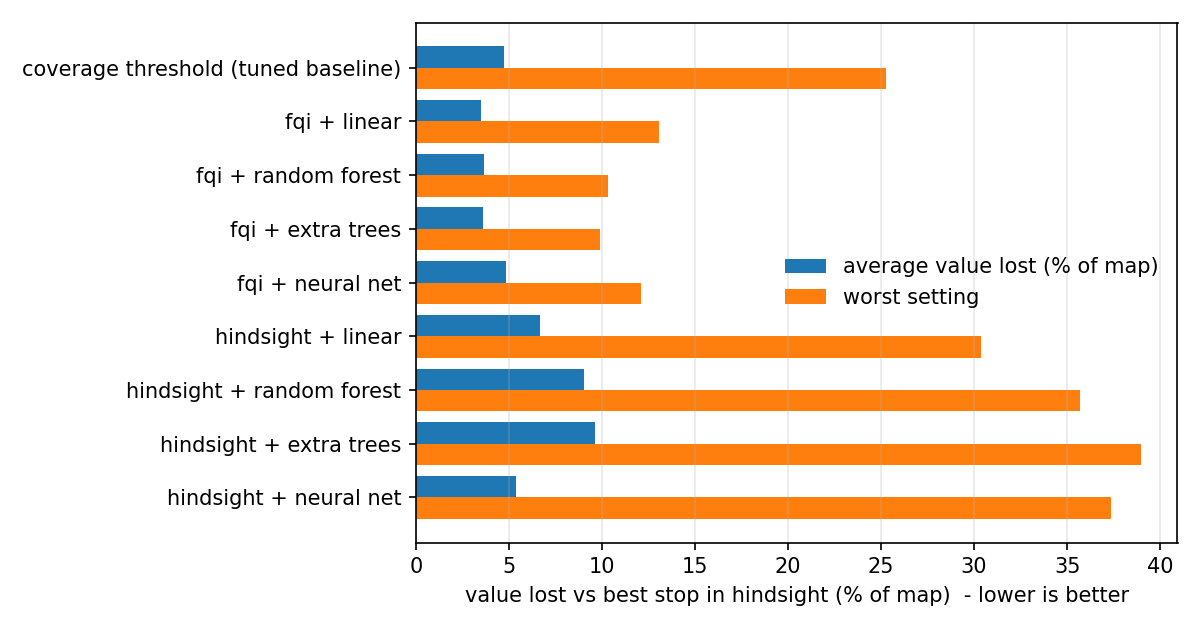
\includegraphics[width=0.82\linewidth]{figures/week2_models.png}
\caption{The same comparison as a chart: average value lost (blue) and the worst setting (orange).}
\label{fig:stageB}
\end{figure}

Two clear lessons:
\begin{enumerate}
  \item \key{How you build the target matters much more than which model you use.} Every RL-style version beats every hindsight version, especially in the worst case (10--13\% lost versus 30--39\%).
  \item \key{A big model is not needed.} Even a straight-line (linear) model does well with the RL-style target. A neural network adds nothing here.
\end{enumerate}

\emph{Why do hindsight answers do worse?} The label says ``this much value was still possible'', but that assumes the team will later stop at exactly the right moment, which it can't, because it doesn't know the future. So the labels are too optimistic, the program thinks continuing is worth more than it is, and it stops too late. People who study stopping problems know this trap; using future knowledge in the targets makes estimates too high \cite{longstaff2001}. The RL-style target only promises what the rule itself can actually deliver.

The learned estimate also tracks reality well: on test maps, its estimate of ``value still left'' has a correlation of 0.88 with the true value, and it gets the basic question ``is it still worth continuing?'' right 89\% of the time.

\subsection{Stage C (so far): how does it compare with the usual rules?}

\begin{table}[h]
\centering
\small
\begin{tabular}{lccc}
\toprule
Stop rule & \% of best & Avg value lost & Worst setting \\
\midrule
\textbf{Learned value-aware stop} & \textbf{91} & \textbf{3.6} & \textbf{9.9} \\
Coverage threshold (tuned) & 92 & 4.7 & 25.3 \\
Gain-vs-cost rule (tuned) & 89 & 6.9 & 15.8 \\
Fixed budget (tuned) & 91 & 9.1 & 37.1 \\
Myopic (stop after a losing cycle) & 68 & 11.4 & 24.5 \\
Explore until done & 74 & 11.4 & 44.6 \\
\bottomrule
\end{tabular}
\caption{``\% of best'' is measured on 140 test maps of the training setting (2 robots, $32\times32$, medium messaging). The other two columns are value lost (\% of map) over the 36 settings, without retraining.}
\label{tab:stageC}
\end{table}

In plain words:
\begin{itemize}
  \item \textbf{In normal cases, it's a tie.} A well-tuned ``stop at 84\% mapped'' rule does as well as my learned rule (92\% vs 91\%).
  \item \textbf{In bad cases, the learned rule is much safer.} Its worst setting loses 9.9\% of the map, against 25.3\% for the coverage rule. That's because a fixed threshold that suits 2 robots doesn't suit 8, while the learned rule adapts without being re-tuned.
\end{itemize}

\subsection{Honest weak spots}
\begin{itemize}
  \item With \textbf{2 robots on the larger maps}, the learned rule sometimes stops 20--33 cycles too early. I don't know why yet; my guess is that it meets situations it never saw in training.
  \item Only \textbf{one type of building} (rooms with furniture). Mazes, warehouses and cluttered spaces are not tested yet.
  \item Only \textbf{one training run}. I need to repeat with several random seeds to make sure the results are not luck.
  \item The \textbf{cost numbers are my choice}, not measured from real robots.
\end{itemize}

% ================================================================
\section{Where the Project Is Heading}

\subsection{From ``when to stop'' to ``how much effort to spend''}

Following the review, the top-level decision changes from a yes/no to a choice of effort level, mainly the number of robots that keep working (and later, how many messages to allow). The value of choosing an effort level $a$ is, in words:
\[
\text{value of } a \;=\; \text{expected extra map from } a \;-\; \text{expected cost of } a
\]
where the cost covers driving, messages, planning and, later, the risk of a robot failing.
The team picks the effort level with the highest value. Stopping (0 robots) is always worth exactly 0, so the team stops when no effort level beats 0. My current rule is just the simplest case of this, with only two choices: continue or stop.

\subsection{Why this needs two levels}

With team size in the picture, there are naturally two decisions at two speeds:
\begin{itemize}
  \item \textbf{Top level (the ``manager''):} once per cycle, decide how many robots keep working and how much they may talk. Zero robots means the mission ends.
  \item \textbf{Bottom level (each robot):} every step, decide where to go, given whoever is still active.
\end{itemize}
This is where multi-agent reinforcement learning (MARL) can come in later: robots that learn to explore together, trained with a method like MAPPO \cite{yu2022mappo}. During training they can use the full map to learn faster, but on a real mission each robot only uses what it can see itself. The idea of a learned ``when to finish'' inside a two-level system comes from hierarchical RL \cite{sutton1999,han2019}.

But, as the review says, MARL is a \emph{tool}, not the contribution. It only gets added once the simpler stages show it is needed.

% ================================================================
\section{The Stage-by-Stage Plan}
\label{sec:plan}

\begin{table}[h]
\centering
\small
\begin{tabularx}{\linewidth}{lXl}
\toprule
Stage & Question & Status \\
\midrule
A & Is the problem real? How much value does exploring until done throw away? & Done \\
B & Can the remaining value be learned? Is RL needed, or is a simple model enough? & Done \\
C & With robot movement fixed, how do all the stopping rules compare, including rules based on the closest papers? & In progress \\
D & Can the team shrink as value drops ($8\to6\to3\to1\to0$) and keep almost the same map for much less cost? & Next \\
E & Two-level learning: a manager that picks team size plus robots that learn where to go (MAPPO). & Next semester \\
\bottomrule
\end{tabularx}
\caption{The staged plan from the review, with where I am.}
\end{table}

\subsection{What I will do for the rest of this semester}

\begin{table}[h]
\centering
\small
\begin{tabularx}{\linewidth}{lXX}
\toprule
When & Build & Output \\
\midrule
Nov, weeks 1--2 & Realistic cost values or a full sweep of costs; three new comparison rules based on Amorín \cite{amorin2019}, Luperto \cite{luperto2026} and PRoID \cite{kim2026proid} & Full Stage C table \\
Nov, weeks 2--4 & Team shrinking (Stage D) & Learned shrinking vs a fixed schedule vs the full team \\
Late Nov & New building types, 5 training seeds, look into the 2-robot failure & Generalisation results \\
Early Dec & Write-up of Stages A--D & Report and an outline of a first paper \\
\bottomrule
\end{tabularx}
\caption{Proposed timeline (to be adjusted to the semester calendar).}
\end{table}

\textbf{Team shrinking (Stage D), in a bit more detail.} Each cycle, the manager picks how many robots stay active. Retired robots stop moving and stop messaging, so they cost nothing. To train it, I will record runs where robots retire at random times, so the program sees every team size, and then use the same fitted Q-iteration with the number of active robots as an extra input. Success would mean: almost the same map value as the full team, at clearly lower driving and messaging cost.

\textbf{Tests decided before training.} The review asked for this explicitly, so the results can't be cherry-picked afterwards:
\begin{itemize}
  \item new building types: maze, warehouse, cluttered;
  \item bigger maps: up to $128\times128$;
  \item bigger teams: train on 2--4 robots, test on 5, 6, 8 and 10;
  \item worse communication: limited range, lost messages, delays;
  \item a sweep of cost settings, to show the trade-off between map value and cost (the review calls this a Pareto analysis).
\end{itemize}

\subsection{Questions I need answered}
\begin{enumerate}
  \item Which cost values are realistic? Should I take them from the robots in the MRTA lab setup, or report a sweep?
  \item When a robot is retired, does it park where it is, or drive back to base (and pay for that trip)?
  \item Is retiring permanent, or can a robot be brought back later?
  \item Is a first paper on value estimation and stopping alone (no MARL) a good first target?
\end{enumerate}

% ================================================================
\section{Papers I Have Been Working With}

The shared literature sheet currently has 33 entries. The target is 50 by the end of November and 80 before the MARL stage starts, each recorded against the review's questions (what decision it makes, learned or hand-made, single robot or team, which costs it counts, and so on). These are the papers that shaped the work so far.

\subsection{Closest work on stopping exploration}
\begin{itemize}
  \item \textbf{Amorín et al.\ 2019} \cite{amorin2019}: a stop rule for a whole robot team based on how much new information the team is still expected to gain. The closest earlier work; it becomes one of my comparison rules.
  \item \textbf{Placed and Castellanos 2022} \cite{placed2022}: one robot stops when its uncertainty about the map and its own position stops improving. A principled rule, but single-robot and it doesn't count driving or messaging costs.
  \item \textbf{Luperto et al.\ 2026} \cite{luperto2026}: a neural network looks at an image of the partial map and says ``explored'' or ``not explored''. Learned, but from labelled examples, single-robot and not cost-aware. Their code is public, so I can compare against it.
  \item \textbf{PRoID (Kim et al.\ 2026)} \cite{kim2026proid}: in a team, each robot decides when to stop exploring and go back to share its data, using a formula. Decided per robot rather than for the team, and not learned.
  \item \textbf{WiSER-X (Jadhav et al.\ 2026)} \cite{jadhav2026wiserx}: robots explore using wireless signals instead of sharing maps, and each one can finish on its own. Relevant to the long-term goal of making the decision without a central controller.
\end{itemize}

\subsection{Where my method comes from}
\begin{itemize}
  \item \textbf{Ernst et al.\ 2005} \cite{ernst2005}: fitted Q-iteration with tree models. This is exactly my training method.
  \item \textbf{Longstaff and Schwartz 2001; Tsitsiklis and Van Roy 1999} \cite{longstaff2001,tsitsiklis1999}: estimating ``the value of continuing'' from data and stopping when it isn't worth it. My stop rule is this idea moved from finance to robots. Becker et al.\ \cite{becker2019} do the same with neural networks.
\end{itemize}

\subsection{Background on exploration and team learning}
\begin{itemize}
  \item \textbf{Yamauchi 1997} \cite{yamauchi1997}: invented frontiers. My robots use them.
  \item \textbf{Burgard et al.\ 2005} \cite{burgard2005}: sending each robot to a different frontier by weighing gain against travel. My robots' movement rule follows this.
  \item \textbf{Tan et al.\ 2023; MARVEL 2025} \cite{tan2023,chiun2025marvel}: recent work where robots \emph{learn} where to go. Their missions end at a fixed time or coverage, which is the gap I'm working on.
  \item \textbf{MAPPO (Yu et al.\ 2022)} \cite{yu2022mappo}: a simple, strong method for training robot teams. The planned method for Stage E.
  \item \textbf{Han et al.\ 2019; Sutton et al.\ 1999} \cite{han2019,sutton1999}: two-level learning where agents learn when to finish a sub-task. Close in spirit, but they end sub-tasks, not the whole mission.
  \item \textbf{Szostak and Cohen 2024} \cite{szostak2024}: a team of agents that learns when to stop collecting samples. A learned team stop, but with no map and no driving.
  \item \textbf{Oliehoek and Amato 2016} \cite{oliehoek2016}: the textbook way to describe a team where each member sees only part of the world. I use it to describe the problem formally.
  \item \textbf{Agarwal et al.\ 2021} \cite{agarwal2021}: how to report learning results fairly. My evaluation follows it.
\end{itemize}

% ================================================================
\section{What I Learned Along the Way}

A few things that were not obvious to me at the start:
\begin{itemize}
  \item \textbf{Check whether the problem is real before solving it.} Stage A showed the problem disappears when driving is cheap. That was humbling, and it changed what I need to do next.
  \item \textbf{The training target matters more than the model.} I expected a neural network to win. Instead, the choice of target decided everything, and a linear model was nearly as good.
  \item \textbf{Average results hide the important part.} The learned rule only ties the best simple rule on average. The real difference shows up in the worst cases.
  \item \textbf{Claims need care.} ``Nobody has done this'' was wrong. A narrower, precise claim is easier to defend and more honest.
\end{itemize}

% ================================================================
\section{Summary}

This semester I built the simulator, the cost model and a learned stop rule, and completed the first two stages of the plan from the review. The problem is real when driving and messaging are expensive, and the RL-style way of learning is clearly needed, while a big model is not. Against the usual stopping rules, the learned rule ties in normal cases and is much safer in bad ones.

Next, I will use realistic costs, compare against rules based on the closest papers, and, most importantly, let the system decide how many robots keep working instead of just when to stop. Two-level learning with MARL comes only if that shows a real gain.

\bibliographystyle{plain}
\bibliography{refs}

\end{document}
